\chapter{Estudio Cinemático y Matemático} \label{chap:Cinematica}
\chapterimage{figuras/ImagenesPortada/PortadaCinematica.jpg}
\hrule
\vspace{3mm}

Este capítulo describe y desarrolla las relaciones matemáticas que definen los aspectos del brazo robótico tal y como se ha descrito, principalmente las relacionadas con la cinemática del robot.

\section{Convenio de ángulos y referencias}

	Antes de comenzar con las ecuaciones matemáticas se deben establecer unas referencias básicas. En la figura \ref{fig:Control:cinematica_3} se pueden ver representadas las que se utilizarán en apartados posteriores.
	
	\begin{itemize}
		\item \textbf{q1, q2 y q3}: ángulo de giro de las articulaciones uno, dos y tres respectivamente. La flecha marca el sentido creciente de los ángulos estando el cero situado en: eje X para el caso de q1 y en el eje vertical para el caso de q2 y q3.
		\item \textbf{Dimensiones del brazo}: siendo conocidas L1, L2, L3, LA, LB.
		\item \textbf{Punto $(x_r,y_r,z_r)$}: extremo del brazo respecto al cual se obtiene la cinemática.
		\item \textbf{Ángulos auxiliares}: q2' y q3' que tendrán un papel importante en cálculos posteriores.
	\end{itemize}
	
	Tal y como se ha explicado en el capítulo \ref{chap:Mecanica} se contempla una variación en el apoyo y/o base del brazo robótico en función del lugar donde se instale. La cinemática está referenciada respecto de la articulación $A_1$, utilizando el sistema de referencia representado en la figura \ref{fig:Control:cinematica_3}.
	
    \begin{figure}[H]
    	\centering
    	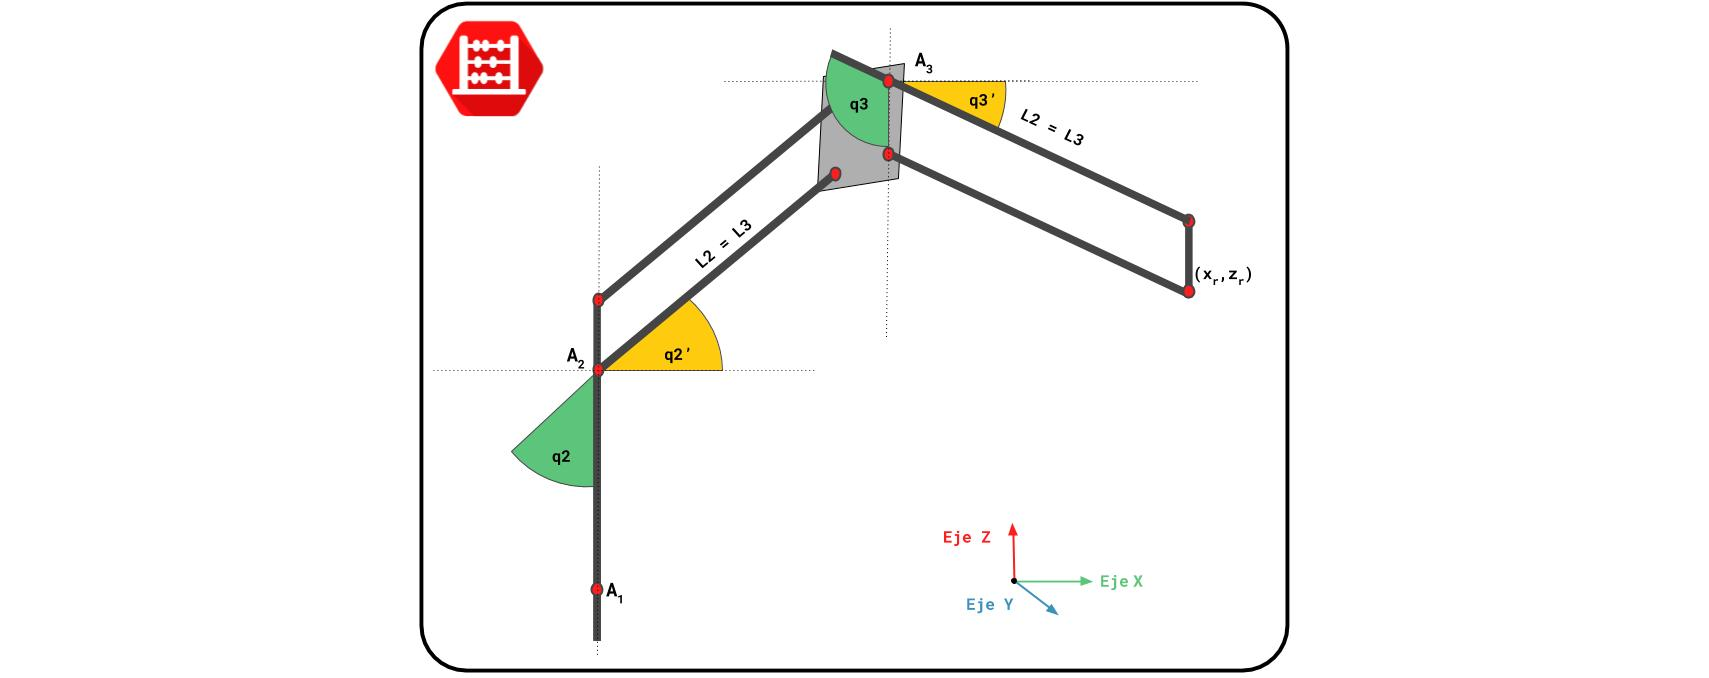
\includegraphics[width=1\textwidth]{figuras/Imagenes_cinematica/cinematica_3.jpg}
    	\caption{Relación con los ángulos y medidas de interés}
    	\label{fig:Control:cinematica_3}
    	\immagesource{Autor}
    \end{figure}
    
    Además de los parámetros descritos el desarrollo de la cinemática utiliza una serie de medidas auxiliares que se pueden ver en la figura \ref{app:codificacionSW} donde es importante destacar la definición del punto $(x_p,y_p,z_p)$.

    \begin{figure}[H]
    	\centering
    	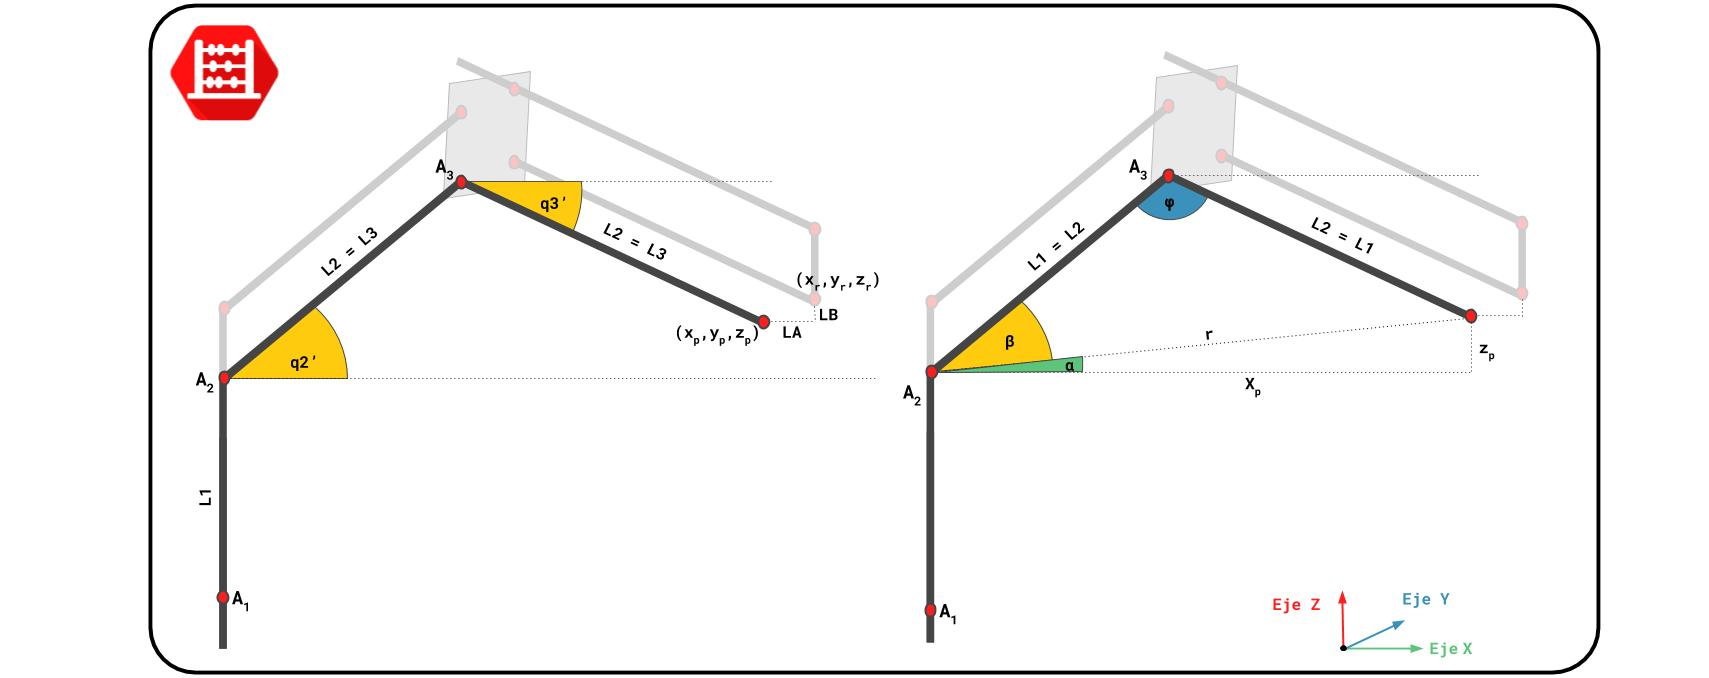
\includegraphics[width=1\textwidth]{figuras/Imagenes_cinematica/cinematica_1.jpg}
    	\caption{Representación de los ángulos y distancias auxiliares más representativas. GDL 2 y 3}
    	\label{fig:Control:cinematica_1}
    	\immagesource{Autor}
    \end{figure}
    
    Las coordenadas \textit{X} y \textit{Z} del punto \textit{p} se obtienen de desplazar el punto \textit{r} simplificar los cálculos angulares. La coordenada en el eje Y coincide para ambos puntos (ver figura \ref{fig:Control:cinematica_2}).
    \begin{figure}[H]
    	\centering
    	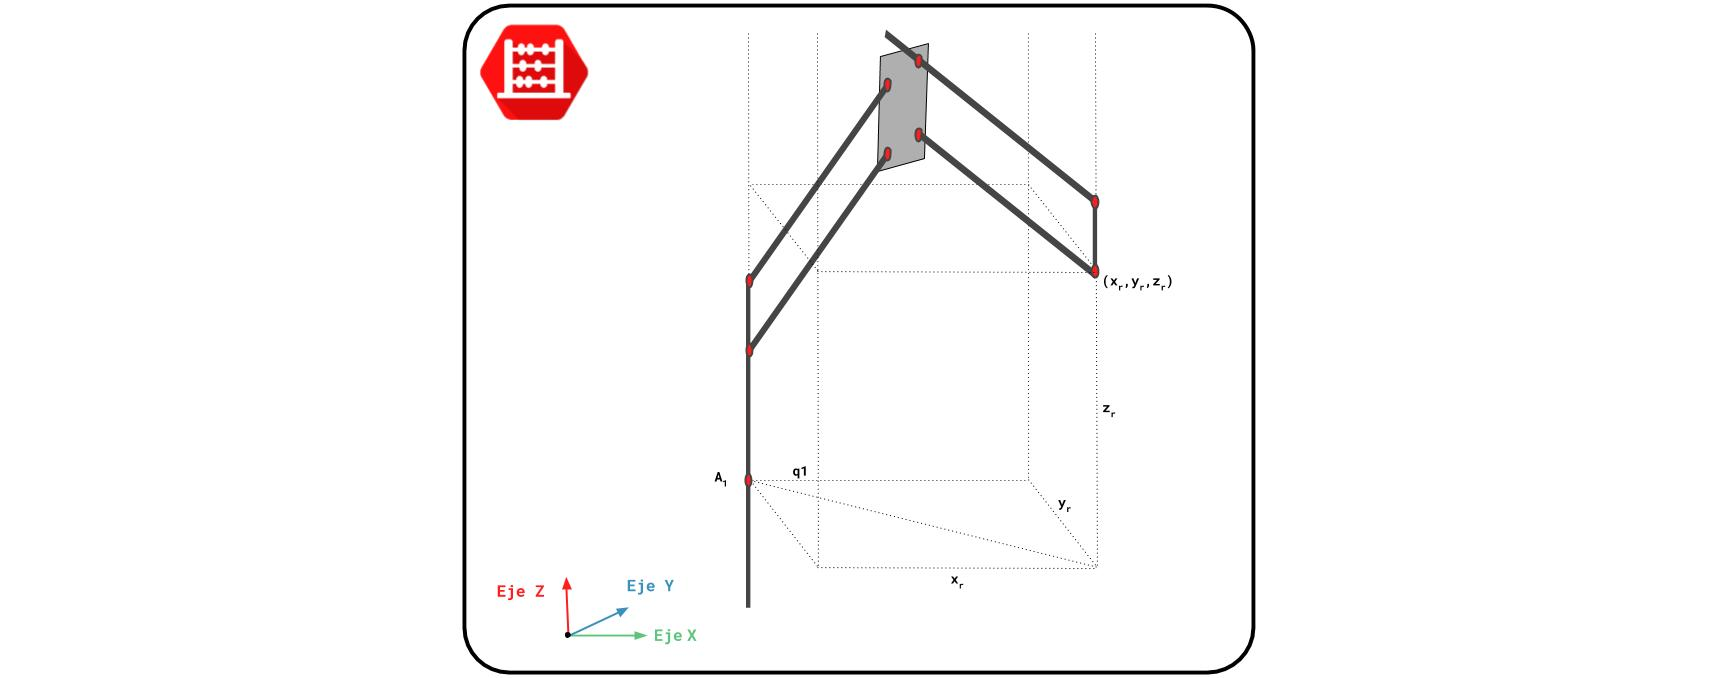
\includegraphics[width=1\textwidth]{figuras/Imagenes_cinematica/cinematica_2.jpg}
    	\caption{Representación de los ángulos y distancias más representativas. Primer grado de libertad}
    	\label{fig:Control:cinematica_2}
    	\immagesource{Autor}
    \end{figure}
\section{Cinemática del robot}

    La solución del problema cinemático del brazo tal y como se ha diseñado es bastante sencilla de obtener mediante métodos geométricos. Aunque se presentan los parámetros de Denavit-Hartenberg y el cálculo definitivo y control del brazo utilizan las relaciones obtenidas mediante relaciones geométricas.
    \\
    
    Como se ha descrito en el capítulo \ref{chap:Mecanica} la orientación de la barra acopladora así como de la barra del extremo se mantienen siempre perpendiculares al plano del suelo; esto permite referenciar los ángulos de las articulaciones dos y tres (d2 y q3 en la figura \ref{fig:Control:cinematica_3}) respecto del eje vertical, de forma que son independientes de la posición angular del resto de articulaciones. Como se verá a continuación esta característica facilita los cálculos matemáticos.
    \\
    
    Las funciones trigonométricas seno, coseno y tangente no son unívocas para giros completos de $360^o$, la cinemática calculada tiene unos rangos de aplicación definidos para cada articulación en base al movimiento que físicamente son capaces de realizar. Se pueden ver estos intervalos en la tabla \ref{tab:rangos_art}.
    
    \begin{table}[H]
    	\caption{Rango de movimiento articular.}
    	\immagesource{Autor}
    	\label{tab:rangos_art}
    		\begin{center}
    			\begin{tabular}{ |c|c|c| }
    				\hline
    				\textbf{Articulación} & \textbf{Extremo inferior} & \textbf{Extremo superior}  \\
    				\hline
    				q1 & $0^o$ & $180^o$ \\
    				\hline
    				q2 & $90^o$ & $180^o$ \\
    				\hline
    				q3 & $0^o$ & $90^o$ \\
    				\hline
    			\end{tabular}
    		\end{center}
    \end{table}

	Las medidas del brazo robótico, presentadas inicialmente en la figura \ref{fig:Control:cinematica_3} pueden verse en la tabla \ref{tab:medidas} , los cálculos de la cinemática mantendrán estas variables de manera simbólica.
	
 \begin{table}[H]
    	\caption{Medidas estructurales}
    	\immagesource{Autor}
    	\label{tab:medidas}
    	\begin{center}
    		\begin{tabular}{ |c|c| }
    			\hline
    			L1 & 0.3270 m \\
    			\hline
    			L2 & 0.455 m \\
    			\hline
    			L3 & 0.455 m \\
    			\hline
    			LA & 0.030 m \\
    			\hline
    			LB & 0.042 m \\
    			\hline
    		\end{tabular}
    	\end{center}
 \end{table}
	    
\subsection{Parámetros de Denavit-Hartenberg}
	Se ha desarrollado siguiendo los pasos descritos por \cite{barrientos}. En la figura \ref{fig:Control:dh} puede verse la posición de los sistemas de referencia definidos. En la tabla \ref{tab:dh} se muestran los parámetros de Denavit-Hartenberg en base a dichos sistemas de referencia. Se calcula respecto al punto \textit{p}, cuya relación posterior con el extremo \textit{r} es directa.
		
	\begin{figure}[H]
		\centering
		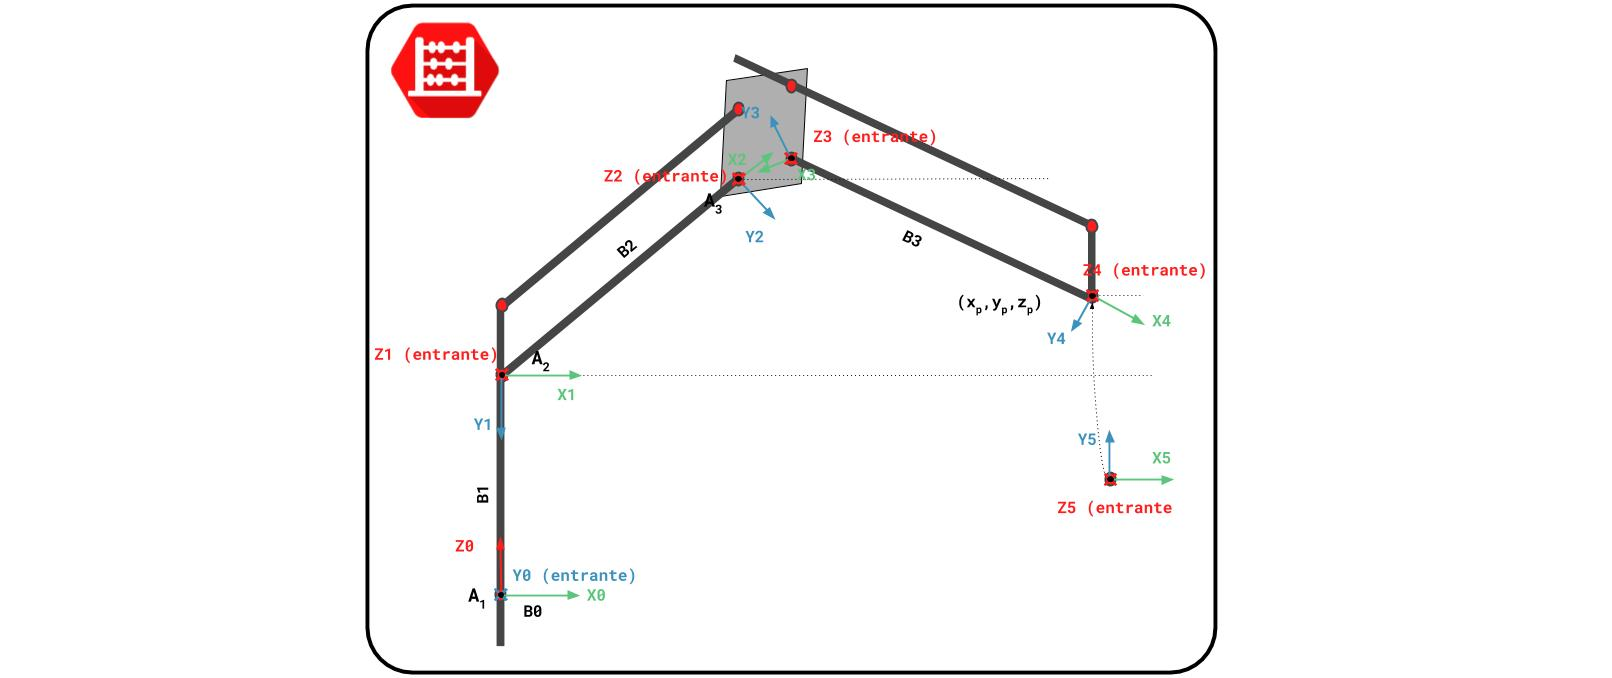
\includegraphics[width=1\textwidth]{figuras/Imagenes_cinematica/denavit-hartemberg_virtuales.jpg}
		\caption{Sistemas de referencia}
		\label{fig:Control:dh}
		\immagesource{Autor}
	\end{figure}
	
	Nótese que los ángulos $q_2$ y $q_3$ a los que se hace referencia en este apartado, los ángulos de los parámetros de Denavit-Hartenberg, son en realidad $q_2'$ y $q_3'$ presentados anteriormente.
	
	 \begin{table}[H]
	 	\caption{Medidas estructurales}
	 	\immagesource{Autor}
	 	\label{tab:dh}
	 	\begin{center}
	 		\begin{tabular}{ |c|c|c|c|c| }
	 			\hline
	 			Articulación & $\Theta$ (grados) & d & a & $\alpha$ (grados)\\
	 			\hline
	 			1 & $q_1$ & L1 & 0 & 90 \\
	 			\hline
	 			2 & $q_2$ & 0 & L2 & 0 \\
	 			\hline
	 			3 (virtual) & $\left(180+q_2-\arctan{\frac{LB}{LA}}\right)$ & 0 & $\sqrt{{LA}^2+{LB}^2}$ & 0 \\
	 			\hline
	 			4 & $\left(\arctan{\frac{LB}{LA}}+q3\right)$ & 0 & L3 & 0 \\
	 			\hline
	 			5 (virtual) & $-q_3$ & 0 & 0 & 0 \\
	 			\hline
	 		\end{tabular}
	 	\end{center}
	 \end{table}
	 
	 Aunque no se muestra el desarrollo completo matricial para resolver la cinemática directa se ha desarrollado una serie de funciones en matlab para resolverla. Se presentan a continuación en el fragmento de código 6.1.
	 
	 \lstset{language=matlab, breaklines=true, basicstyle=\footnotesize}
	     \begin{lstlisting}[frame=single, caption=Cálculos con DH en matlab, label=code:dhmatlab]
function [dh] = denavith_Aij(theta,d_i,a_i,alfa_i)
	syms theta_i %d_i a_i alfa_i	
	theta_i=theta;	
	dh = [cos(theta_i),-cosd(alfa_i)*sin(theta_i),sind(alfa_i)*sin(theta_i),a_i*cos(theta_i);sin(theta_i),cosd(alfa_i)*cos(theta_i),-sind(alfa_i)*cos(theta_i),a_i*sin(theta_i);0,sind(alfa_i),cosd(alfa_i),d_i;0,0,0,1];	
end

%%%%%%%%%%%%%%%%%%%%%%%%%%%%%%%

function Dirkinematics	
	syms th1 th2 th3 L1 L2 L3	
	
	% Parametros Denavit-Hartenberg del robot	
	teta = [th1 90+th2 90+th3 0];	
	d = [0 L1 0 L3];	
	a = [0 0 L2 0];	
	alfa = [0 90 0 0];	
	
	% Matrices de transformacion homogenea entre sistemas de coordenadas consecutivos	
	A01 = denavith_Aij( teta(1),d(1),a(1),alfa(1) );	
	A12 = denavith_Aij( teta(2),d(2),a(2),alfa(2) );	
	A23 = denavith_Aij( teta(3),d(3),a(3),alfa(3) );	
	A34 = denavith_Aij( teta(4),d(4),a(4),alfa(4) );	
	
	% Matriz de transformacion del primer al ultimo sistema de coordenadas	
	T04 = A01*A12*A23*A34;
		
	%Coordenadas posicion ejes cartesianos	
	PX = T04(1,4);	
	PY = T04(2,4);	
	PZ = T04(3,4);	
end
	     \end{lstlisting}
	
\subsection{Cinemática directa}
	Siendo conocidos las posiciones articulares de los tres grados de libertad se puede obtener la posición en coordenadas cartesianas del punto \textit{r} definido respecto al punto A1. Se definen primero algunos puntos intermedios sobre los que se apoya el cálculo:
	\\
	
	Ángulos auxiliares q2' y q3':
	 \begin{equation}
	 \label{cd:eq1}
	 q2' = q2 - \frac{\varPi}{2}
	 \end{equation}
	 \begin{equation}
	 \label{cd:eq2}
	 q3' = \frac{\varPi}{2} - q3 
	 \end{equation}
	 Conviene también recordar de la tabla \ref{tab:medidas} la relación siguiente:
	 \begin{equation}
	 \label{cd:eq3}
	 L1 = L2
	 \end{equation}
	
	Apoyándose en las relaciones de \ref{cd:eq1}, \ref{cd:eq2} y \ref{cd:eq3} se obtiene la cinemática directa del brazo robótico:
	    
    \begin{equation}
    x_r = x_p+LA = \cos(q1)\left(LA + L2 \cdot \left(\cos(q2') + \cos(q_3')\right)\right)
    \end{equation}
    
    \begin{equation}
    y_r = y_p = \sin(q1)\left(LA + L2 \cdot \left(\cos(q2') + \cos(q_3')\right)\right)
    \end{equation}
    
    \begin{equation}
    z_r = z_p+LB+L1 = LB + L1 + L2\cdot\left( \sin(q2') - \sin(q3') \right)
    \end{equation}
\subsection{Cinemática inversa}

	Siendo conocida la posición del extremo (punto \textit{r}) en coordenadas cartesianas se calcula la posición angular de cada articulación. Se definen algunas relaciones sobre las que se apoyará el cálculo matemático.
	\\
	
	Se definen las coordenadas X y Z del punto \textit{p} de la siguiente manera: 
	\begin{equation}
	\label{ci:eq0}
	x_p = \sqrt{x_r^2+y_r^2} - LA
	\end{equation}
	\begin{equation}
	\label{ci:eq1}
	y_p = y_r
	\end{equation}
	\begin{equation}
	\label{ci:eq2}
	z_p = z_r - LB - L1
	\end{equation}
	
	La diagonal r representada en la figura \ref{fig:Control:cinematica_1}:
	\begin{equation}
	\label{ci:eq31}
	r = \sqrt{x_p^2+y_p^2}
	\end{equation}
	
	
	Además se utilizan los ángulos auxiliares descritos a continuación:
	\begin{equation}
	\label{ci:eq3}
	\alpha = \arctan\left(\frac{z_p}{x_p}\right)
	\end{equation}
	
	\begin{equation}
	\label{ci:eq4}
	\beta = \arccos\left(\frac{r^2+L2^2-L3^2}{2 \cdot L2 \cdot r}\right) = \arccos\left(\frac{r}{2 \cdot L2}\right)
	\end{equation}
	
	\begin{equation}
	\label{ci:eq5}
	\varphi = \arccos\left(\frac{L2^2+L3^2-r^2}{2 \cdot L2 \cdot L3}\right) = \arccos\left(\frac{r}{2L2}\right)
	\end{equation}
	
	\begin{equation}
	\label{ci:eq6}
		q2' = \alpha + \beta
	\end{equation}
	
	\begin{equation}
	\label{ci:eq7}
		q3' = \varPi - q2' - \varphi
	\end{equation}
	
	Finalmente, apoyándose sobre las relaciones descritas (y recordando las ecuaciones \ref{cd:eq1} y \ref{cd:eq2}) se obtiene las relaciones cinemáticas para obtener las posiciones articulares conociendo el punto del extremo: 
	 \begin{equation}
	 \label{ci:eq8}
	 q1 = \arctan\left(\frac{y_p}{x_p}\right)
	 \end{equation}
	 
	 \begin{equation}
	 \label{ci:eq9}
	 q2 = \frac{\varPi}{2} - q2'
	 \end{equation}
	 
	 \begin{equation}
	 \label{ci:eq10}
	 q3 = q3'- \frac{\varPi}{2}
	 \end{equation}
\subsection{Cinemática diferencial}
	 Por derivación de las relaciones de la cinemática directa se puede obtener la relación entre las velocidades articulares y la velocidad del extremo, el punto \textit{r}. De forma matricial se puede expresar esta relación de la siguiente manera:
	\begin{equation}
		\label{cdif:eq0}
		\left[ \begin{array}{c}
			\dot x_r \\
			\dot y_r \\
			\dot z_r \\
		\end{array}\right]
		=
		\left[ \begin{array}{ccc}
		N_{11} & N_{12} & N_{13} \\
		N_{21} & N_{22} & N_{23} \\
		N_{31} & N_{32} & N_{33} \\
		\end{array}\right]
		\cdot
		\left[ \begin{array}{c}
		\dot q_1 \\
		\dot q_2 \\
		\dot q_3 \\
		\end{array}\right]
	\end{equation}
	Teniendo los valores $N_{xx}$ la siguiente forma:
	 \begin{equation}
	 \label{cdif:eq1}
	 N_{11} = \frac{\partial x_r}{\partial q_1}
	 \end{equation}
 	 \begin{equation}
 	 \label{cdif:eq2}
 	 N_{33} = \frac{\partial z_r}{\partial q_3}
 	 \end{equation}
 	 
	Se ha desarrollado un \textit{script} en matlab para resolver esta serie de cálculos de manera simbólica, puede verse en el fragmento de código 6.2.
	
		 \lstset{language=matlab, breaklines=true, basicstyle=\footnotesize}
		 \begin{lstlisting}[frame=single, caption=Cálculo cinemática diferencial, label=code:diferencialmatlab]
	%Cinematica diferencial
	
	syms q1 q2 q3 l2 l1 a b
	
	q2_transf = q2 - pi/2;
	q3_transf = pi/2 - q3;
	
	xp = cos(q1)*(a + l2*cos(q2_transf) + l2*cos(q3_transf));
	yp = sin(q1)*(a + l2*cos(q2_transf) + l2*cos(q3_transf));
	zp = b + l2*sin(q2_transf) - l2*sin(q3_transf) + l1;
	
	N11 = diff(xp,q1)
	N12 = diff(xp,q2)
	N13 = diff(xp,q3)
	
	N21 = diff(yp,q1)
	N22 = diff(yp,q2)
	N23 = diff(yp,q3)
	
	N31 = diff(zp,q1)
	N32 = diff(zp,q2)
	N33 = diff(zp,q3)
		 \end{lstlisting}
		 
 	 Obteniéndose los siguientes resultados:
 	 
	\begin{equation}
	N_{11} = - \sin\!\left(\mathrm{q1}\right)\, \left(a + \mathrm{l2}\, \cos\!\left(\mathrm{q2} - \frac{\pi}{2}\right) + \mathrm{l2}\, \cos\!\left(\mathrm{q3} - \frac{\pi}{2}\right)\right)
	\end{equation}
	\begin{equation}
	N_{12} = - \mathrm{l2}\, \cos\!\left(\mathrm{q1}\right)\, \sin\!\left(\mathrm{q2} - \frac{\pi}{2}\right)
	\end{equation}
	\begin{equation}
	N_{13} = - \mathrm{l2}\, \cos\!\left(\mathrm{q1}\right)\, \sin\!\left(\mathrm{q3} - \frac{\pi}{2}\right)
	\end{equation}

 	 
 	 \begin{equation}
 	 N_{21} = \cos\!\left(\mathrm{q1}\right)\, \left(a + \mathrm{l2}\, \cos\!\left(\mathrm{q2} - \frac{\pi}{2}\right) + \mathrm{l2}\, \cos\!\left(\mathrm{q3} - \frac{\pi}{2}\right)\right)
 	 \end{equation}
 	 \begin{equation}
 	 N_{22} = - \mathrm{l2}\, \sin\!\left(\mathrm{q1}\right)\, \sin\!\left(\mathrm{q2} - \frac{\pi}{2}\right)
 	 \end{equation}
 	 \begin{equation}
 	 N_{23} = - \mathrm{l2}\, \sin\!\left(\mathrm{q1}\right)\, \sin\!\left(\mathrm{q3} - \frac{\pi}{2}\right)
 	 \end{equation}

 	 
 	 \begin{equation}
 	 N_{31} = 0
 	 \end{equation}
 	 \begin{equation}
 	 N_{32} = \mathrm{l2}\, \cos\!\left(\mathrm{q2} - \frac{\pi}{2}\right)
 	 \end{equation}
 	 \begin{equation}
 	 N_{33} = \mathrm{l2}\, \cos\!\left(\mathrm{q3} - \frac{\pi}{2}\right)
 	 \end{equation}

	\begin{landscape}
	 	 Una vez resuelto matemáticamente el cálculo de todos los valores de $N_{xx}$ y sustituyendo en la ecuación \ref{cdif:eq0} se obtiene la siguiente relación:
	 	 
		\begin{equation}
		\left[ \begin{array}{c}
		\dot x_r \\
		\dot y_r \\
		\dot z_r \\
		\end{array}\right]
		=
		\left[ \begin{array}{ccc} - \sin\!\left(\mathrm{q1}\right)\, \left(a + \mathrm{l2}\, \cos\!\left(\mathrm{q2} - \frac{\pi}{2}\right) + \mathrm{l2}\, \cos\!\left(\mathrm{q3} - \frac{\pi}{2}\right)\right) & - \mathrm{l2}\, \cos\!\left(\mathrm{q1}\right)\, \sin\!\left(\mathrm{q2} - \frac{\pi}{2}\right) & - \mathrm{l2}\, \cos\!\left(\mathrm{q1}\right)\, \sin\!\left(\mathrm{q3} - \frac{\pi}{2}\right)\\ \cos\!\left(\mathrm{q1}\right)\, \left(a + \mathrm{l2}\, \cos\!\left(\mathrm{q2} - \frac{\pi}{2}\right) + \mathrm{l2}\, \cos\!\left(\mathrm{q3} - \frac{\pi}{2}\right)\right) & - \mathrm{l2}\, \sin\!\left(\mathrm{q1}\right)\, \sin\!\left(\mathrm{q2} - \frac{\pi}{2}\right) & - \mathrm{l2}\, \sin\!\left(\mathrm{q1}\right)\, \sin\!\left(\mathrm{q3} - \frac{\pi}{2}\right)\\ 0 & \mathrm{l2}\, \cos\!\left(\mathrm{q2} - \frac{\pi}{2}\right) & \mathrm{l2}\, \cos\!\left(\mathrm{q3} - \frac{\pi}{2}\right) \end{array}\right]
		\cdot
		\left[ \begin{array}{c}
		\dot q_1 \\
		\dot q_2 \\
		\dot q_3 \\
		\end{array}\right]
		\end{equation}
	\end{landscape}
	
\subsection{Rango de movimientos}
	Con los limites angulares definidos se obtiene un espacio de trabajo de brazo robótico (para el plano de trabajo XZ, en la posición y=0). Tal y como puede apreciarse en la figura \ref{fig:cinematica:espacioTrabajo}, este espacio de trabajo es suficiente para el objetivo que se desea dar. Abarca una distancia óptima para alcanzar los diferentes puntos a lo ancho de una camilla pudiendo posicionar la tablet a diferentes alturas. Para obtener el espacio de trabajo tridimensional solo hay que girar el espacio obtenido en el plano XZ al rededor del eje Z, para abarcar los $180^o$ que gira la primera articulación.
	
	 \begin{figure}[H]
	 	\centering
	 	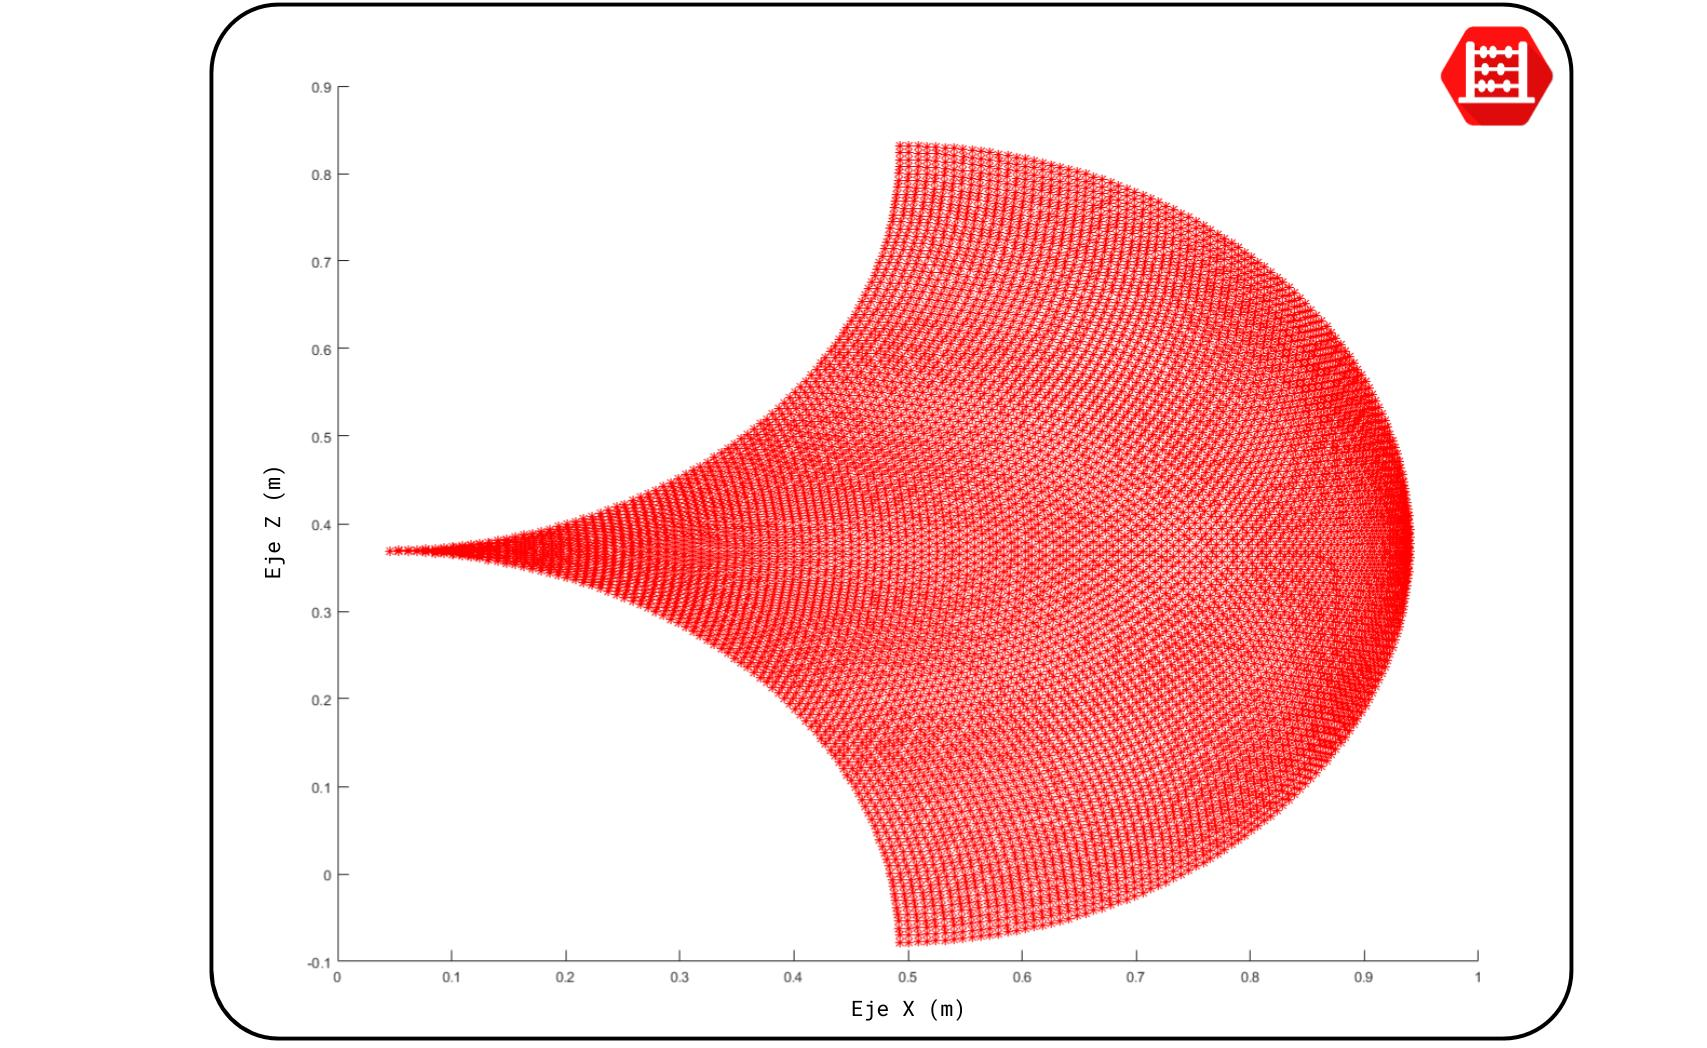
\includegraphics[width=\textwidth]{figuras/Imagenes_cinematica/workspace_robot.jpg}
	 	\caption{Espacio de trabajo en el plano XZ para Y = 0}
	 	\label{fig:cinematica:espacioTrabajo}
	 	\immagesource{Autor.}
	 \end{figure}
\section{Realimentación articular}

	La relación entre las medidas angulares de los potenciómetros y de las articulaciones varían de una a otra. En ambos casos una vez transformado a ángulo articular habrá que aplicar el desfase para posicionar el cero angular en las posiciones descritas en la figura \ref{fig:Control:cinematica_3}. Hay que recordar de la sección \ref{sec:Electronica:Integracion} de qué manera se han integrado los potenciómetros en la estructura.
	
	   \begin{equation}
		   \textnormal{Segunda articulación:} \to	angulo_{articulacion} = angulo_{potenciometro} 
	   \end{equation}
	   
	   \begin{equation}
		   \textnormal{Tercera articulación:} \to	   angulo_{articulacion} = angulo_{potenciometro} \cdot 0.679
	   \end{equation}
